\chapter{Interpolazione - Laplace}

Siano $x_0, x_1, \dots, x_n$, $n + 1$ \textbf{punti distinti} e siano $L_0(x), L_1(x), \dots, L_n(x)$ polinomi di grado $n$ tali che:
\begin{equation}
 L_j(x_i) = \delta_{j, i} = 
   \begin{cases}
      1 \quad se \quad i = j \\ 
      0 \quad se \quad i \neq j
   \end{cases}
   \quad 
   i = 0,1, \dots, n
\end{equation}

Dove:
\begin{equation}
  L_n(x) = \prod_{k=n,k\neq n}^{n} \displaystyle\frac{x - x_k}{x_n - x_k}
\end{equation}



Trovare la funzione interpolatrice dati i seguenti voncoli
\begin{center}
  \begin{tabular}{ c c c }
    $x_0$ & $x_1$ & $x_2$ \\
    $y_0$ & $y_1$ & $y_2$ \\
    $y_0'$
  \end{tabular}
\end{center}

Quinsi devo usare costruire il sistema:
\begin{equation}
  \begin{cases}
    a_0 + a_1x_0 + a_2x_0^2 + a_3x_0^3 = y_0 \\
    a_1 + 2a_2x_0^1 + 3a_3x_0^2 = y_0' \\
    a_0 + a_1x_1 + a_2x_1^2 + a_3x_1^3 = y_1 \\
    a_0 + a_1x_2 + a_2x_2^2 + a_3x_2^3 = y_2
  \end{cases}
\end{equation}

E poi da qui posso risolvere il sistema.

\section{Polinomio di Newton}

Si chiama differenza divisa di ordine $k$ della funzione $f(x)$ relativa ai punti $x_0, \dots, x_{k-1}$
la funzione $f[x_0, \dots, x_{k-1}, x]$ defiinita per $x \neq x_i$ con $i = 0, \dots, k-1$ ricorsivamente come:

\begin{figure}[h!]
  \begin{center}
    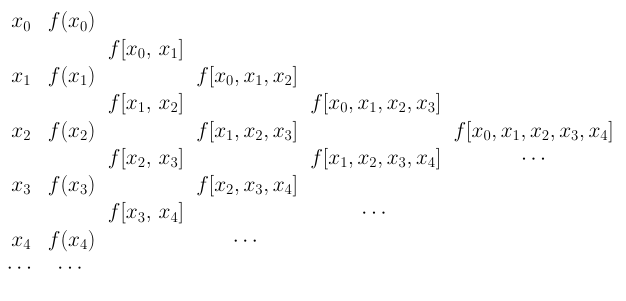
\includegraphics[width=0.5\textwidth]{./images/newton.png}
  \end{center}
  \caption{Schema iterazione polinomio Newton}
  \label{fig:iterazione_newton}
\end{figure}


Per calcolare il polinomio finale di Newton si deve iterare come segue:

Se siamo nella prima colonna(dove ci sono gli $x_n$):
\begin{equation}
  f[x] = f(x)
\end{equation}

Se ci troviamo nella colonna 1(dove si trovano $f(x_n)$), prendo due x alla volta e eseguo:
\begin{equation}
  f[x_0, x_1] = \displaystyle\frac{f[x] - f[x_0]}{x - x_0}
\end{equation}

Se mi trovo nelle colonne dalla numero 2 in poi (andando verso destra):
\begin{equation}
  f[x_0, \dots, k_{k-2}, x_{k-1}, x] = \displaystyle\frac{f[x_1, \dots, x_{k-1}, x] - f[x_0, \dots, x_{k-1}, x_{k-1}]}{x - x_0}
\end{equation}

Il polnomio ottenuto con Newton è al più di grado $n$, nel polinomio interpolatore di newton, i coefficienti $[x_0, \dots, x_n]$ sono indipendenti da $x$.

\subsection{Polinomio interpolatore lineare}
\begin{equation}
  p_1(x) = f[x_0] + (x - x_0) \displaystyle\frac{f(x_1) - f(x_0)}{x_1 - x_0}
\end{equation}

\subsection{Polinomio interpolatore quadratico}
\begin{equation}
  p_2(x) = f[x_0] + (x - x_0) f[x_0, x_1] + (x - x_0)(x - x_1) f[x_0, x_1, x_2]
\end{equation}

\subsection{Algoritmo di Horner}
Algoritmo ottimale per calcolare un polinomio in un punto:
% \begin{equation}
%   p_n(x) = a_0 + a_1x a_2x^2 + \dots + a_{n-1}x^{n-1} + a_nx^n
% \end{equation}
% Si può riscrivere coem:
% \begin{equation}
%   p_n(x) = (\dots (((a_nx + a_{n-1})x + a_{n-2})x + a_{n-3})\dots)x + a_0
% \end{equation}

Il polinomio:
\begin{equation}
  p(x) = a_0 + a_1x + a_2x^2 + a_3x^3
\end{equation}
Si può riscrivere come:
\begin{equation}
  p(x) = ((a_3x + a_2)x + a_1)x + a_0
\end{equation}


\subsection{Newton con derivate(Hermite)}
Se i punti $f(x)$ appartengon all'intervallo chiuso e limitato $[a, b]$, non necessariamente distinti,
esiste un punto $\epsilon$ compreso tra il minimo e il massimo tale che:
\begin{equation}
  f[x_0, \dots, x_k] = \displaystyle\frac{f^{(k)}\epsilon}{k!}
\end{equation}


Se si conoscono anche le derivate prime di $f(x)$ si può fare:

\begin{figure}[h!]
  \begin{center}
    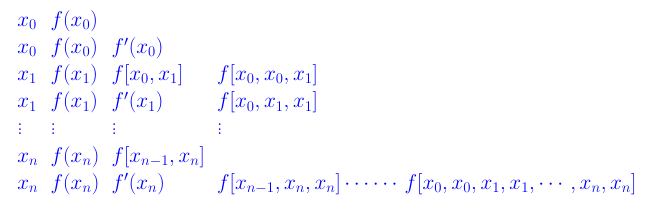
\includegraphics[width=0.5\textwidth]{./images/hermite.png}
  \end{center}
  \caption{Hermite}
  \label{fig:hermite}
\end{figure}



Esempio:
Se nel punto $x_0$ ho tre vincoli:
\begin{itemize}
  \item $f(x)$
  \item $f'(x)$
  \item $f''(x)$
\end{itemize}

Posso realizzare lo schema delle differenze divise come:
\begin{figure}[h!]
  \begin{center}
    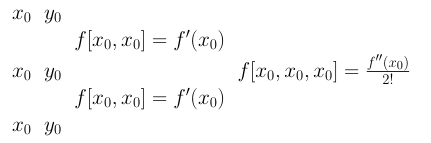
\includegraphics[width=0.5\textwidth]{./images/esempio_hermite.png}
  \end{center}
  \caption{Esempio hermite}
  \label{fig:esempio_hermite}
\end{figure}


Il polinomio risulta cosi:
\begin{equation}
  p(x) = f[x_0] + f[x_0, x_0](x - x_0) + f[x_0, x_0, x_0](x-x_0)^2
\end{equation}


\section{Interpolazione inversa}
Se la funzione da interpolare $f(x)$ è:
\begin{itemize}
  \item monotona in senso stretto in $[a, b]$
\end{itemize}
quindi è invertibile, la formula di interpolazione di Newton può essere usata per ottenere 
l'inversa.

Basta scambiare i punti $x, y$.

Esempio:
Dati i seguenti punti:

\begin{center}
  \begin{tabular}{c | c c c c}
    $x_i$ & $0.2$ & $0.4$ & $0.6$ & $0.8$ \\
    $f(x_i)$ & $0.203$ & $0.423$ & $0.684$ & $1.030$
  \end{tabular}
\end{center}


\begin{center}
  \begin{tabular}{c | c c c c}
    $y_i$ & $0.203$ & $0.423$ & $0.684$ & $1.030$ \\
    $x_i = f^{-1}(y_i)$ & $0.2$ & $0.4$ & $0.6$ & $0.8$ 
  \end{tabular}
\end{center}


